\begin{figure*}
  \begin{center}
    \begin{tabular}{c}
      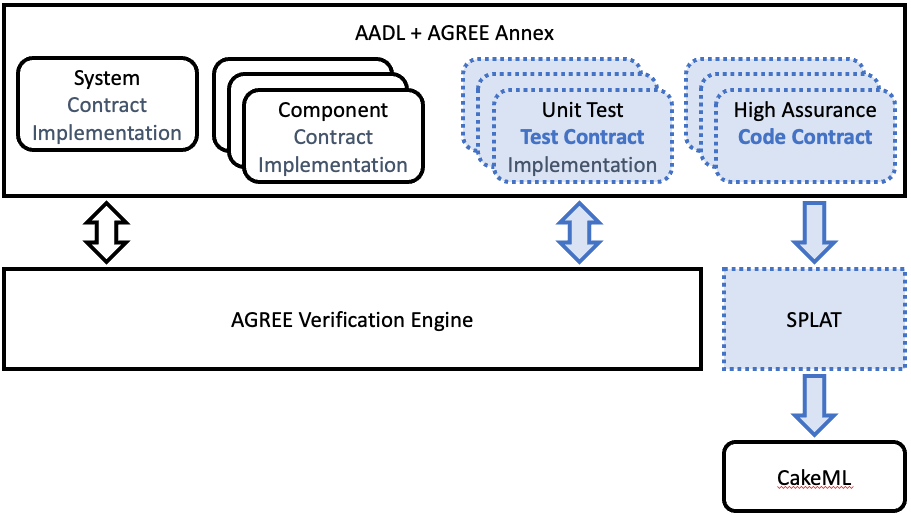
\includegraphics[scale=0.4]{flowchart.png} \\
    \end{tabular}
  \end{center}
\caption{Simplified \brfcs\ workflow. Shaded portions are the focus of the present discussion.}
\label{fig:flowchart}
\end{figure*}

\begin{figure*}[h]
  \begin{center}
    \begin{tabular}{c}
      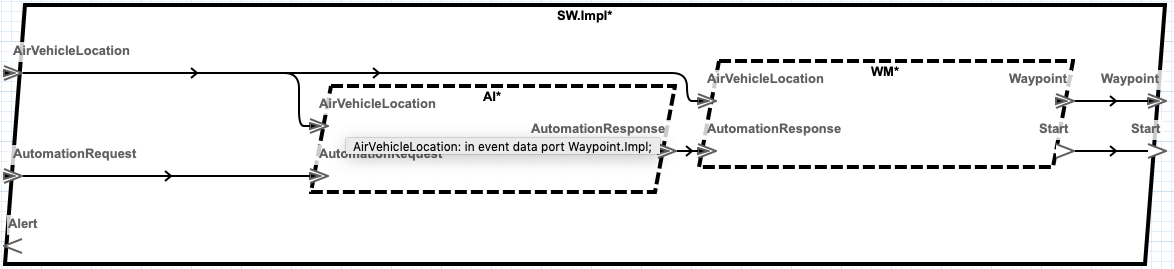
\includegraphics[scale=0.4]{example.png}
    \end{tabular}
  \end{center}
\caption{Initial design for an automated UAV route planning system.}
\label{fig:example}
\end{figure*}

\begin{figure}
  \begin{center}
    \begin{tabular}{c}
      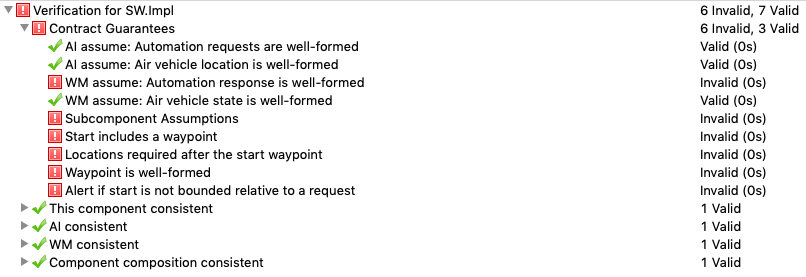
\includegraphics[scale=0.4]{example-certificate.png} \\
    \end{tabular}
  \end{center}
\caption{\agr\ failure certificate for initial design.}
\label{fig:example-certificate}
\end{figure}

\figref{fig:flowchart} illustrates a simplified \brfcs\ workflow with the shaded boxes representing our focus: test contracts, code contracts, and SPLAT synthesis.
The unshaded boxes are the existing tools that generate evidence for the assurance case.
The rest of this section follows an illustrative example through the workflow.

The baseline AADL model is a simple software system, named SW, for route planning
and automated control of a UAV. A picture of the architectural
model for SW is in \figref{fig:example}. SW is loosely based on
the case study in \secref{sec:case-study}.  The source for the
entire model is found at \cite{repo}.

From time to time, SW receives a message on the \texttt{AutomationRequest} input,
forwarding it to a route planner (AI). The function of AI is to
compute the flight path (a list of waypoints) for the UAV, outputting
the resulting \emph{mission command} on \texttt{AutomationResponse}.
The waypoint manager (WM) receives the mission command from AI and
starts the UAV flying the mission by putting an \emph{event} on the
\texttt{Start} output port, continuing to issue waypoints to the UAV
flight controller on the \texttt{Waypoint} port as the UAV location
updates with messages on \texttt{AirVehicleLocation}.
%%An event is repeatedly generated on \texttt{Alert} if there is no
%%mission command from a request.
The AI component is third-party
software and WM is a legacy component.

%% that cannot be modified so it critically relies on
%% assumptions about its input behavior to guarantee its intended output
%% behavior.

The expected behavior of the SW system, and the components
implementing the system, are modeled with \agr\ contract
specifications.
These contracts assume and guarantee the absence
of any malicious, or unspecified, component behavior.  More precisely,
the contract for SW assumes that its inputs are \emph{well-formed} and that
there is never more than one automation request pending at a time.
Well-formed generally refers to a syntactic restriction on
data at a port. For example, a waypoint is well-formed if it falls
within bounds for latitude, longitude, and altitude.  The guarantees
for SW ensure that
\begin{compactitem}
\item a start coincides with a new waypoint being output;
\item a start is within one cycle of an automation request and if not, then it persistently alerts;
\item new waypoints coincide with location updates; and
\item all outputs are well-formed.
\end{compactitem}

The contracts for the sub-components assume their inputs are
well-formed, and they guarantee their outputs are well-formed.  The AI
contract guarantees it only responds to automation requests and always
in the same cycle.  The legacy WM contract guarantees that
\begin{compactitem}
  \item it generates a start from a response from the AI and always in the same cycle;
  \item the start coincides with a waypoint; and
  \item any further waypoints coincide with location updates.
\end{compactitem}

These initial specifications pass verification, meaning that the
contract composition of the components with the system satisfies all
component input assumptions and system output guarantees.
The \agr\ verification conditions, syntax and semantics, and the baseline contracts for the example are discussed in detail in \secref{sec:agree}.

\subsection{Adding cyber requirements}

A cyber-vulnerability analysis identifies the potential of a
supply chain attack through the AI route planner since its third-party.  Based on the analysis, the designer adds a requirement that the system must guard against malicious AI behavior.
They additionally remove all output guarantees from its contract since it is untrusted.

The output from the \agr\ analysis is shown in \figref{fig:example-certificate}.  The red
exclamation points designate component assumptions or system output
guarantees that do not hold, and each failure comes with a
corresponding counter-example.  The first violation is that the mission command on \texttt{AutomationResponse} from
the AI to the WM is no longer guaranteed to be well-formed.  The
consequence of that failing input assumption is that the WM outputs
are no longer guaranteed.  These
missing guarantees lead to the rest of the failures
in \figref{fig:example-certificate} as the WM provides the system
level outputs.

\begin{figure*}
  \begin{center}
    \begin{tabular}{c}
      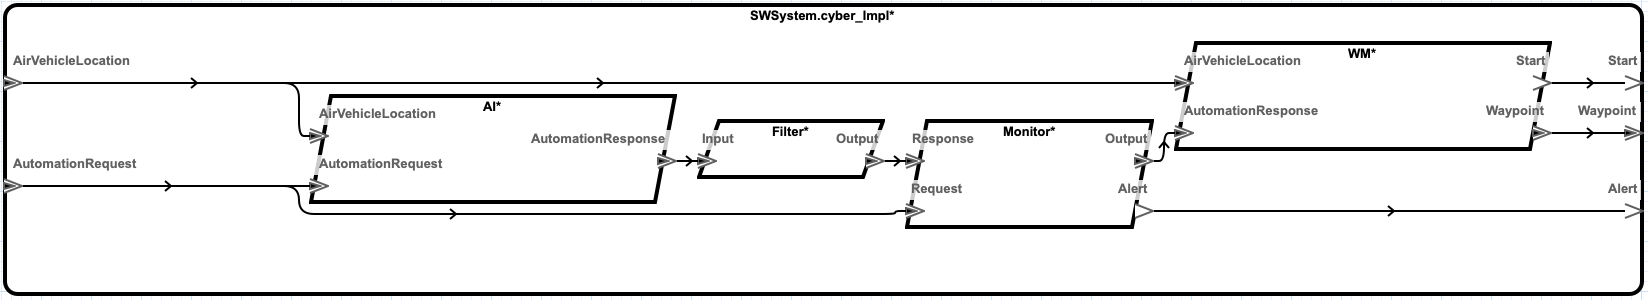
\includegraphics[scale=0.3]{hardened.png}
    \end{tabular}
  \end{center}
  \caption{Cyber-hardened design for an automated UAV route planning system}
  \label{fig:hardened}
\end{figure*}

\begin{figure}
  \begin{center}
    \begin{tabular}{c}
      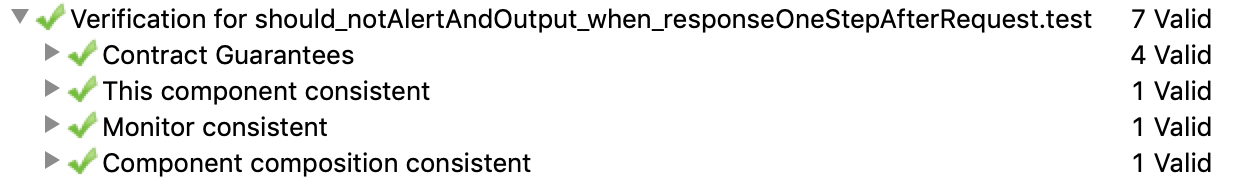
\includegraphics[scale=0.38]{agree-test-output.png} \\
      (a) \\ \\
      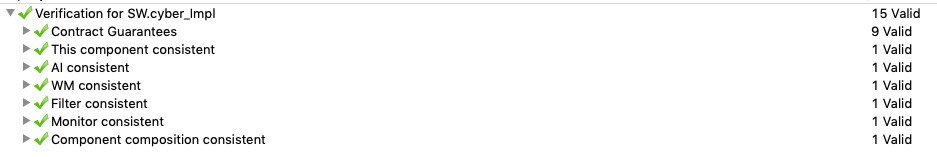
\includegraphics[scale=0.4]{hardened-certificate.png} \\
      (b)
    \end{tabular}
  \end{center}
  \caption{\agr\ verification certificates. (a) Test contract verification results. (b) Cyber-hardened design verification results.}
  \label{fig:hardened-certificate}
\end{figure}

\subsection{Adding high assurance components}

Here is where the shaded regions in \figref{fig:flowchart} come into play.
The system designer now uses \brfcs\ to cyber-harden SW by inserting
high-assurance components in the form of a filter and a monitor, as
shown in \figref{fig:hardened}.
These are intended to mitigate and report any observed malicious behavior by AI.

A filter enforces an invariant over
each datum in the data stream by not forwarding input to its output if the invariant does not hold.
\brfcs\ generates an initial code contract for the filter which the designer completes by writing the invariant.
That invariant is usually based on the existing assumptions made by
downstream components that consume the filter output.
In this example, it is the well-formed property for the automation request.

A monitor captures a relation on data over time and is thus able
to reason about the temporal, and other invariant, properties of that data.  It raises
an alert if the specified properties are ever violated.
As with the filter, \brfcs\ generates an initial code contract that is completed by the designer.
In this example, that contract states that an
automation response can only be generated in conjunction with an
automation request; and further, that response must come with the
request or in the next step after the request.
Code contracts are discussed in detail in \secref{sec:code-contracts}.

Code contracts for high assurance components can be arbitrarily complex since they can have persistent state that evolves over time.
Test contracts allow the designer to validate code contract behavior with unit testing.
For example, one of the test contracts for the monitor is that when it sees an automation response one step after a request, then it should not alert, and it should pass the response downstream.
Test contracts are discussed in detail in \secref{sec:testing}.

The \agr\ analysis of the cyber-hardened implementation is shown in
\figref{fig:hardened-certificate}.
\figref{fig:hardened-certificate}(a) is the test contract results and \figref{fig:hardened-certificate}(b) is the hardened system composition.
Here \agr\ has generated high-level
evidence justifying the claim that the high-assurance components meet their intended purposes.
Having passed \agr\ verification, the high-assurance components are ready to be
synthesized.

\subsection{Synthesizing code from code contracts}

High-assurance components are automatically synthesized by \splt\ from
the code contracts to equivalent programs in the \ckml\ language.  In
other words, for any set of input streams that meet the component's
contract assumptions, the output streams produced from the synthesized
\ckml\ code exactly match those defined by the contract guarantees.
As such, the \agr\ verification results regarding the code contract
apply equally to the synthesized \ckml, and thus, the results equally
apply to the resulting binaries from the \ckml\ compiler.  Synthesis
from code contracts is discussed in detail in \secref{sec:synthesis}.

Extending the \agr\ verification results to the system composition
requires additional guarantees not discussed here.  For
example, among other things, contracts for non-synthesized components
must be certified to accurately model their deployed counterparts, the
HAMR generated scheduler must be certified to follow the dependent
data-flow in the design, scheduling windows must be certified to cover
worst-case execution times, \etc.  Such additional guarantees are
discussed in other works \cite{gearcase2020, dcrypps2019,
  10.1007/978-3-030-89159-6_18, 10.1007/978-3-030-89159-6_17,
  sel4-2009, scheduled-agree, 9734792}.
